\documentclass[openany,12pt,a4paper]{report}
\usepackage{subfiles}
\usepackage[]{graphicx}
\usepackage{float}
\usepackage{multirow}
\graphicspath{{./img/}{./../img/}}
\usepackage{../StileDoc}
\title{Manuale Utente}
\author{}

\loadglsentries{../Glossario/Definizioni}
%Ultima versione documento

\newcommand{\versione}{0.0.0}


\begin{document}
	\makeatletter
	\begin{titlepage}
		\setlength{\headsep}{0pt}  
		\begin{center}
			
\includegraphics[width=0.5\linewidth]{img/logo.png}\\[1em]
			{\huge \bfseries  \@title }\\[10ex]
			\textbf{\Large Informazioni Documento} \\[2em]
			\bgroup
			\def\arraystretch{1.5}
			\begin{tabular}{l|l}
				\textbf{Versione} & \versione{} \\
				\textbf{Data approvazione} & 10 Marzo 2018 \\
				\textbf{Responsabile} & Marco Focchiatti\\
				\textbf{Redattori} &  Manfredi Smaniotto, Marco Focchiatti,\\
				& Cristiano Tessarolo, Giulio Rossetti \\
				\textbf{Verificatori} & Manfredi Smaniotto, Marco Focchiatti \\
				\textbf{Distribuzione} & Prof. Tullio Vardanega \\
				& Prof. Riccardo Cardin \\
				& Mivoq S.R.L. \\
				& Gruppo Graphite \\
				\textbf{Uso} & Esterno \\
				\textbf{Recapito} & graphite.swe@gmail.com \\
			\end{tabular}
			\egroup
		\end{center}
	\end{titlepage}
	\makeatother
	
	\thispagestyle{empty}
	\newpage
	
	%REGISTRO DELLE MODIFICHE (nella versione 0.0.0 non è stato inserito)
	\begin{comment}
	\chapter*{Registro delle modifiche}
	\setlength\LTleft{-22mm}
	\begin{longtable}{|p{20mm}|p{20mm}|p{40mm}|p{30mm}|p{50mm}|}
		\hline
		\textbf{Versione} & \textbf{Data} & \textbf{Autore} & \textbf{Ruolo} & \textbf{Descrizione} \\
		
		\hline 2.0.0 & 10-03-2018 & Marco Focchiatti & Responsabile & Approvazione \\
		\hline 1.2.0 & 09-03-2018 & Giulio Rossetti & Verificatore & Verifica \\
		\hline 1.1.1 & 08-03-2018 & Kevin Silvestri & Verificatore & Stesura appendice §C.3 e §D  \\
		\hline 1.1.0 & 25-02-2018 & Marco Focchiatti & Verificatore & Verifica \\
		\hline 1.0.6 & 23-02-2018 & Manfredi Smaniotto & Verificatore & Stesura appendice §B \\
		\hline 1.0.5 & 22-02-2018 & Manfredi Smaniotto & Verificatore & Spostamento appendice §B in appendice §C \\
		\hline 1.0.4 & 16-02-2018 & Giulio Rossetti & Verificatore & Rivisto e modificato §3 \\
		\hline 1.0.3 & 13-02-2018 & Cristiano Tessarolo & Verificatore & Rivisti obiettivi di qualità (§2.2) e aggiunta politica della qualità (§2.4) \\
		\hline 1.0.2 & 11-02-2018 & Kevin Silvestri & Verificatore & Spostate definizioni metriche (§3) in NP\\
		\hline 1.0.1 & 09-02-2018 & Marco Focchiatti & Verificatore & Rivista struttura generale e ampliata §2 \\
		\hline 1.0.0 & 12-01-2018 & Samuele Modena & Responsabile & Approvazione \\
		\hline 0.2.0 & 11-01-2018 & Giulio Rossetti & Verificatore & Verifica \\
		\hline 0.1.2 & 10-01-2018 & Samuele Modena & Verificatore & Stesura appendice §B \\
		\hline 0.1.1 & 20-12-2017 & Matteo Rizzo & Verificatore & Aggiornata §3 \\
		\hline 0.1.0 & 19-12-2017 & Manfredi Smaniotto & Verificatore & Verifica \\		
		\hline 0.0.6 & 18-12-2017 & Kevin Silvestri & Verificatore & Stesura appendice §A \\
		\hline 0.0.5 & 17-12-2017 & Kevin Silvestri & Verificatore & Stesura §4 \\	
		\hline 0.0.4 & 15-12-2017 & Matteo Rizzo & Verificatore & Stesura §3 \\
		\hline 0.0.3 & 14-12-2017 & Samuele Modena & Verificatore & Stesura §2 \\
		\hline 0.0.2 & 13-12-2017 & Matteo Rizzo & Verificatore & Stesura §1 \\
		\hline 0.0.1 & 13-12-2017 & Matteo Rizzo & Verificatore & Creazione del template \\
		\hline
		
	\end{longtable}
	\end{comment}
	
	% INDICE
	\tableofcontents
	
	% INTRODUZIONE
	
	\chapter{Introduzione}
	
	\section{Scopo del documento}
	
	Il documento ha la finalità di spiegare le funzionalità e le modalità di utilizzo dell’applicazione
	\textit{"DeSpeect: un'interfaccia grafica per Speect"}. Nonostante la versione attuale rappresenti una prima bozza del documento, una volta concluso esso rappresenterà sia una guida che un riferimento completo per l’utilizzo del prodotto da parte di un utente.
	
	\section{Scopo del prodotto}
	
	Lo scopo del progetto è la realizzazione di un’interfaccia grafica per \glossario{Speect}{Speect} [Meraka Institute(2008-2013)], una libreria per la creazione di sistemi di sintesi vocale, che agevoli l’ispezione del suo stato interno durante il funzionamento e la scrittura di test per le sue funzionalità.
	
	\section{Informazioni utili}
	
	La stesura di questo documento assume come utente target del prodotto un programmatore esperto nell'utilizzo di \textit{Speect} e dei linguaggi di programmazione C e C++. \\
	\noindent Per completezza, viene riportato in appendice A un glossario comprensivo di termini tecnici o riguardanti particolari funzionalità di \textit{DeSpeect}. Per identificare i termini presenti nel glossario, la loro prima occorrenza all’interno del documento è riportata in corsivo e marcata con una G al pedice. 
	
	%quando caricheremo su github in una repo apposita il manuale sviluppatore
	\begin{comment}
	\\ \noindent Per i manutentori del prodotto o per chi fosse interessato alla sua integrazione/incremento, può invece consultare il manuale sviluppatore reperibile all'indirizzo: \url{...}
	\end{comment}
	
	\section{Riferimenti informativi}

	\begin{itemize}
		\item \textbf{Documentazione Speect:} \\
		\url{http://speect.sourceforge.net/contents.html};
		\subitem Documentazione ufficiale della libreria di \textit{Text-To-Speech} di riferimento per il progetto.
		
		\item \textbf{Documentazione Qt:} \\
		\url{http://doc.qt.io/};
		\subitem Documentazione ufficiale del framework utilizzato per lo sviluppo dell'interfaccia grafica.
		
		\item \textit{Documentazione CMAKE:} \\
		\url{https://cmake.org/documentation/}.
		\subitem Documentazione ufficiale del framework utilizzato per la build del prodotto. 
	\end{itemize}

	\chapter{Requisiti di sistema}
	L'installazione ed esecuzione del software DeSpeect richiede i seguenti prerequisiti:
	
	\begin{itemize}
		\item Sistema operativo Unix / Unix-like (il software è stato testato solo per piattaforma Ubuntu 16.04 LTS)
		\subitem \url{https://www.ubuntu.com/download/desktop}
		\item CMake (versione minima 2.8)
		\subitem \url{https://cmake.org/download/}
		\item Compilatore ANSI C/ISO C90 GCC (versione minima 5.0)
		\subitem \url{https://gcc.gnu.org/install/binaries.html}
		\item Qt 5.9.0
		\subitem \url{https://www.qt.io/download}
	\end{itemize}	
	 
	\chapter{Installazione e configurazione} 
	
	DeSpeect è reperibile su \glossario{GitHub}{GitHub} al seguente link:
	\begin{center}
		\url{https://github.com/graphiteSWE/DeSpeect}
	\end{center}
	
	\noindent Una volta soddisfatti i prerequisiti descritti in §2 "Requisiti di sistema" di questo documento, per installare ed eseguire il software è necessario seguire la seguente procedura:
	\begin{enumerate}
		\item Clonare o scaricare la repository sulla propria macchina;
		\item Entrare nella cartella scaricata ed eseguire lo script \verb|build.sh|.
	\end{enumerate}
	Tale procedura installerà la libreria Speect e genererà una build del software nella directory \verb|DeSpeect/build|, nonché avvierà automaticamente un'esecuzione di DeSpeect.
	
	\chapter{Guida all'utilizzo}
	Di seguito è presentata una guida all'utilizzo di DeSpeect.
	I termini evidenziati in \textbf{questo modo} corrispondono a pulsanti presenti all'interno dell'applicazione.
	
	\section{Interfaccia grafica}
	All'avvio dell'applicazione viene presentata una schermata come in Figura 1.
	\begin{figure}[H]
		
		\centering
		
		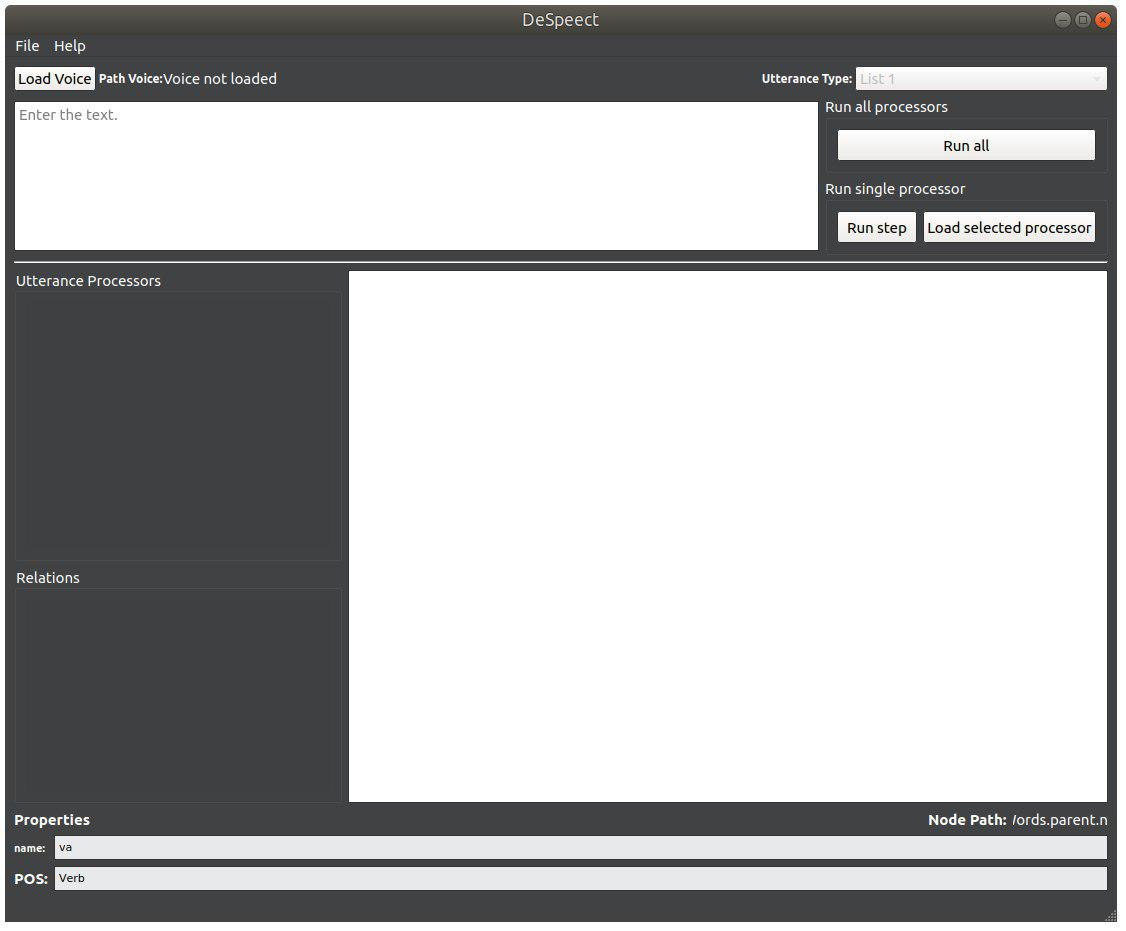
\includegraphics[width=\textwidth]{./img/avvio.png}
		
		\caption{Interfaccia grafica - pagina iniziale}
		
	\end{figure}
 	L'interfaccia grafica sarà sempre generalmente composta dalle seguenti componenti:
 	\begin{itemize}
 		\item 
 	\end{itemize}
	
	\subsection{Struttura dell'interfaccia grafica}
	
	\subsection{Visualizzare il manuale utente}
	
	\subsection{Uscire dall'applicazione}
	
	\section{Interagire con la voice}
	
	\subsection{Caricare la voice}
	
	\subsection{Generare l'audio relativo alla voice}
	
	\subsection{Salvare l'audio relativo alla voice}
	
	\section{Stampare il grafo}
	
	\subsection{Importare il grafo}
	
	\subsection{Selezionare gli utterance processors}
	
	\subsection{Visualizzare il grafo}
	
	\subsubsection{Visualizzare il grafo step-by-step}
	
	\subsubsection{Visualizzare l'intero grafo}
	
	\section{Interagire con il grafo}
	
	\subsection{Esportare il grafo generato}
	
	\subsection{Traslare elementi grafici}
	
	\subsubsection{Traslare nodi}
	
	\subsubsection{Traslare archi}
	
	\subsection{Interagire con le relation}
	
	\chapter{Risoluzione dei problemi}
	
	\section{Errori in DeSpeect}
	
	\subsection{Struttura dei codici di errore}
	
	\subsection{Log degli errori}
	
	\section{Problemi con il reperimento di Speect}
	
	\section{Segnalazione di bug}
	
	\textit{DeSpeect} potrebbe contenere bug o potrebbe essere desiderabile apportare modifiche e ampliamenti alle sue funzionalità. \\ È possibile segnalare malfunzionamenti o richieste di nuove funzionalità sotto forma di GitHub issue all’indirizzo:
	\begin{center}
		\url{https://github.com/graphiteSWE/DeSpeect}
	\end{center}
  oppure scrivendo direttamente all'indirizzo e-mail:
  \begin{center}
  	\url{graphite.swe@gmail.com}
  \end{center}
	
	\appendix
	
	\chapter{Glossario}
	
\end{document}
